\documentclass[journal]{IEEEtran}

\usepackage[utf8]{inputenc}
\usepackage{amsmath,amssymb,amsfonts}
\usepackage{algorithmic}
\usepackage{graphicx}
\usepackage{textcomp}
\usepackage{xcolor}
\usepackage{booktabs}
\usepackage{tabularx}
\usepackage{array}
\usepackage{url}
\usepackage{hyperref}

\hypersetup{
    colorlinks=true,
    linkcolor=blue,
    citecolor=blue,
    urlcolor=blue
}

\begin{document}

\title{An Empirical Multi-Layer LLM Architecture for Context-Aware Software Requirement Quality Analysis and Evolutionary Benchmarking}

\author{Akshat$^{1}$,~\IEEEmembership{Student Member,~IEEE,} and Humendra~Narayan$^{2}$%
\thanks{$^{1}$Akshat and $^{2}$Humendra Narayan are with the Department of Computer Science and Engineering (e-mail: akshat@example.org, humendra@example.org).}}

\markboth{IEEE Transactions on Software Engineering,~Vol.~XX, No.~X, October~2026}%
{Akshat and Narayan: Multi-Layer LLM Architecture for Requirement Quality Analysis}

\maketitle

% =========================================================================
% ABSTRACT
% =========================================================================
\begin{abstract}
Natural language Software Requirements Specifications (SRS) remain the principal medium for stakeholder-developer communication, yet informal text is inherently prone to ambiguity, incompleteness, non-singularity, and inconsistency. Recent applications of generative Large Language Models (LLMs) to Requirements Engineering (RE) largely rely on single-shot rewriting, a paradigm that frequently introduces hallucinated technical details, silently alters functional business scope, and flags spurious quality defects due to the absence of surrounding document context. We present SQAM, an ISO/IEC/IEEE 29148:2018-compliant framework that reframes automated requirement quality improvement as a multi-stage surgical editing problem rather than monolithic generative rewriting. The architecture coordinates a five-layer pipeline: multidimensional scoring across seven formal ISO 29148 quality dimensions, contextual false-positive elimination referencing glossaries and neighboring requirements, surgical refinement preserving domain vocabulary and functional intent, fail-closed adversarial validation, and human-in-the-loop decision diffing. To evaluate the framework without relying on lexical-overlap metrics (such as BLEU or ROUGE), which correlate poorly with requirements engineering judgment, we develop a companion Historical SRS Version Evolution Benchmark. This benchmark aligns requirements across chronological releases ($V_N$ vs. $V_{N+1}$) using exact identifiers and TF-IDF cosine similarity fallback ($\ge 0.45$), classifies modifications across a nine-category empirical taxonomy, and evaluates semantic correspondence via qualitative chain-of-thought reasoning. Evaluated across 215 systematically sampled requirements spanning 43 document versions in 15 real-world multi-domain projects, the framework reduces the Flawed Suggestion Rate to 4.2\% (a 34.2-percentage-point reduction relative to single-shot GPT-4o), increases User Acceptance to 88.1\% (+48.2\% over baseline), achieves a 97.6\% Intent Preservation Rate, and enforces 100.0\% deterministic sequence adherence with zero schema escapes across live Model Context Protocol interception and adversarial fuzzing.
\end{abstract}

\begin{IEEEkeywords}
Requirements Engineering, Large Language Models, ISO/IEC/IEEE 29148, Requirements Quality, Software Requirements Specification, Hallucination Mitigation, Adversarial Validation, Empirical Software Engineering.
\end{IEEEkeywords}

% =========================================================================
% SECTION 1: INTRODUCTION
% =========================================================================
\section{Introduction}
\label{sec:introduction}

\IEEEPARstart{N}{atural} language remains the primary vehicle through which stakeholders, domain experts, and software engineers communicate system intent during the requirements phase of the software development lifecycle. This reliance on informal natural language is a double-edged design decision: it maximizes accessibility to non-technical stakeholders, but it inherits the ambiguity, incompleteness, and non-singularity that characterize unconstrained human language. The ISO/IEC/IEEE 29148:2018 standard for requirements engineering processes~\cite{iso29148} codifies a rigorous set of quality criteria---unambiguity, completeness, consistency, conformance, correctness, singularity, and verifiability/feasibility---that a well-formed requirement statement should satisfy. In practice, however, manual inspection of an SRS document against these criteria is labor-intensive, inconsistently applied across reviewers, and scales poorly as document size and system complexity grow, particularly in safety-critical programs where vague or non-verifiable requirements can propagate downstream into design and certification defects.

\subsection{Limitations of Existing LLM Solutions in RE}
\label{sec:limitations}

The recent proliferation of generative LLMs has motivated a wave of tooling applying these models directly to requirements quality tasks~\cite{ronanki2023requirements}. We identify three interrelated limitations in prevailing approaches:

\textbf{1. The Single-Shot Rewriting Trap.} The dominant pattern among existing LLM-based RE tools is to present a requirement statement to the model and request, in a single inference call, an ``improved'' or ``rewritten'' sentence. In mission-critical software domains, this pattern is hazardous: because the model lacks mechanisms to constrain output to minimal edits, wholesale rewriting frequently introduces unwarranted architectural assumptions (e.g., inventing specific network protocols or data rates), silently contracts or expands functional scope, and alters contractual obligations without explicit notification to human reviewers.

\textbf{2. The Contextual False-Positive Paradox.} A requirement statement read in isolation frequently appears to violate ISO/IEC/IEEE 29148 quality attributes when, in fact, the apparent defect is fully resolved elsewhere in the specification. Consider the statement: \textit{``The system shall respond upon detecting a Vital Anomaly.''} In isolation, ``Vital Anomaly'' appears to be an undefined, ambiguous concept. However, if the SRS glossary explicitly defines \textit{``Vital Anomaly: Systolic pressure $> 180$\,mmHg or HR $< 40$\,bpm,''} flagging this statement as ambiguous constitutes an invalid false positive that wastes engineering effort. Context-free LLM analysis is structurally incapable of distinguishing this class of false positive from genuine defects.

\textbf{3. Flawed Lexical Evaluation (The BLEU/ROUGE Fallacy).} A substantial portion of prior RE research evaluates automatically generated requirement edits using n-gram overlap metrics such as BLEU and ROUGE~\cite{reiter2018structured,sulem2018bleu}. These metrics are structurally unsuited to requirements engineering. An edit that transforms \textit{``The system shall respond quickly''} into \textit{``The system shall respond within 200\,ms''} has near-zero lexical overlap with an equally valid human edit such as \textit{``Response time shall not exceed 250\,ms,''} despite both addressing the identical underlying defect (unquantified latency) with comparable engineering rigor. Penalizing such edits on lexical grounds measures surface-level string similarity rather than requirements quality.

\subsection{Research Questions}
\label{sec:rqs}

This work is structured around three research questions:
\begin{itemize}
    \item \textbf{RQ1 (Contextual Precision):} To what extent does explicit, context-aware defect reasoning (Layer~2) reduce false-positive quality flags relative to context-free, single-shot LLM analysis?
    \item \textbf{RQ2 (Intent and Scope Preservation):} Does the introduction of an independent adversarial auditor layer (Layer~4) effectively eliminate hallucinated technical assumptions, specification drift, and unauthorized functional-scope modification in LLM-proposed requirement refinements?
    \item \textbf{RQ3 (Empirical Historical Fidelity):} How accurately do the automated quality refinements produced by the five-layer pipeline anticipate the actual empirical edits that human software stakeholders subsequently made across chronological SRS releases of the same document?
\end{itemize}

\subsection{Summary of Contributions}
\label{sec:contributions}

This paper makes the following contributions:
\begin{enumerate}
    \item \textbf{A Modular Five-Layer Requirements Quality Pipeline (Pipeline~1):} A surgical requirements editor enforcing ISO/IEC/IEEE 29148:2018 compliance with explicit contextual false-positive filtering prior to text modification.
    \item \textbf{A Context-Aware Defect Reasoning Engine:} A dedicated reasoning stage that grounds candidate defects against project glossaries, domain summaries, and neighboring requirements before defect remediation.
    \item \textbf{A Historical Version Evolution and Alignment Benchmark (Pipeline~2):} A companion benchmark combining exact-identifier matching with TF-IDF cosine-similarity fallback and a nine-category empirical change taxonomy, evaluating semantic correspondence via qualitative chain-of-thought analysis.
    \item \textbf{An Empirical Multi-Domain Corpus Study:} An empirical evaluation spanning 15 versioned SRS projects across 10 engineering domains, verified via a Model Context Protocol (MCP) diagnostics server.
\end{enumerate}

% =========================================================================
% SECTION 2: RELATED WORK
% =========================================================================
\section{Related Work}
\label{sec:related-work}

\subsection{Traditional Rule-Based and Linguistic RE Tools}
\label{sec:related-traditional}

Prior to the widespread availability of generative LLMs, automated requirements quality analysis relied on rule-based natural language processing pipelines~\cite{ferrari2017nlp}. Tools such as QuARS (Quality Analyzer for Requirements Specifications)~\cite{fantechi2002quars}, ARM (Automated Requirement Measurement)~\cite{wilson1997arm}, and Circe~\cite{ambriola1997circe} apply part-of-speech tagging, hand-crafted linguistic pattern dictionaries, and gazetteers of weak phrases, vague adjectives, and optionality markers to flag candidate quality defects. While computationally inexpensive and deterministic, these tools share structural limitations: they cannot reason over document-wide context, exhibit high false-alarm rates on domain-specific terminology, and cannot synthesize contextually appropriate remediations, leaving the remediation burden entirely on the human reviewer~\cite{arora2015automated}.

\subsection{Generative LLMs in Requirements Engineering}
\label{sec:related-llm}

The emergence of instruction-tuned generative LLMs has motivated applied work on requirements generation, test-case synthesis, and user-story classification~\cite{white2023prompt,ronanki2023requirements}. The prevailing methodological pattern treats the LLM as a single-shot generator: a requirement is presented in a prompt, and the model's single response is treated as the final artifact. This literature exhibits a consistent structural gap: it largely lacks formal multi-stage verification gates between generation and human sign-off, leaving pipelines unable to reliably prevent scope drift, hallucinated technical details, or spurious defect flagging.

\subsection{Semantic Evaluation vs. Lexical Overlap in RE}
\label{sec:related-evaluation}

A separate strand of related work critiques n-gram lexical-overlap metrics (BLEU, ROUGE, METEOR) when applied to technical and formal language synthesis tasks~\cite{reiter2018structured,sulem2018bleu}. These metrics were designed for machine translation and summarization, where surface-level phrasing similarity to a reference is a proxy for quality. Empirical studies have reported zero or negative correlation between BLEU scores and practitioners' qualitative acceptance judgments, because a technically correct and stylistically distinct rewording is penalized identically to an incorrect one whenever both diverge lexically from reference text. This finding directly motivates our qualitative semantic correspondence methodology.

% =========================================================================
% SECTION 3: PROPOSED FRAMEWORK
% =========================================================================
\section{Proposed Framework: Dual-Pipeline Architecture}
\label{sec:proposed-framework}

The framework comprises two cooperating pipelines: \textbf{Pipeline~1}, the In-Situ Five-Layer Surgical Requirements Quality Analyzer (Section~\ref{sec:pipeline1}), and \textbf{Pipeline~2}, the Historical SRS Version Evolution Benchmark (Section~\ref{sec:pipeline2}).

\subsection{Overall System Architecture}
\label{sec:architecture-overview}

The high-level architecture separates in-situ quality analysis from historical empirical benchmarking:
\begin{itemize}
    \item \textbf{Pipeline 1 (In-Situ Analyzer):} Operates on an individual requirement within its enclosing SRS document context ($V_N$), producing an audited, reviewable refinement.
    \item \textbf{Pipeline 2 (Evolution Benchmark):} Validates Pipeline~1 by comparing its independent proposals against ground-truth modifications codified in the official Final Version of the SRS ($V_{\text{final}}$ / $V_{N+1}$).
\end{itemize}
The pipelines maintain separation of concerns: the evolution pipeline encapsulates the quality analyzer, orchestrating it against baseline specifications ($V_N$) without leaking future release data ($V_{N+1}$) into the analyzer.

\subsection{Pipeline 1: Five-Layer Surgical Quality Analyzer}
\label{sec:pipeline1}

\begin{figure}[htbp]
\centering
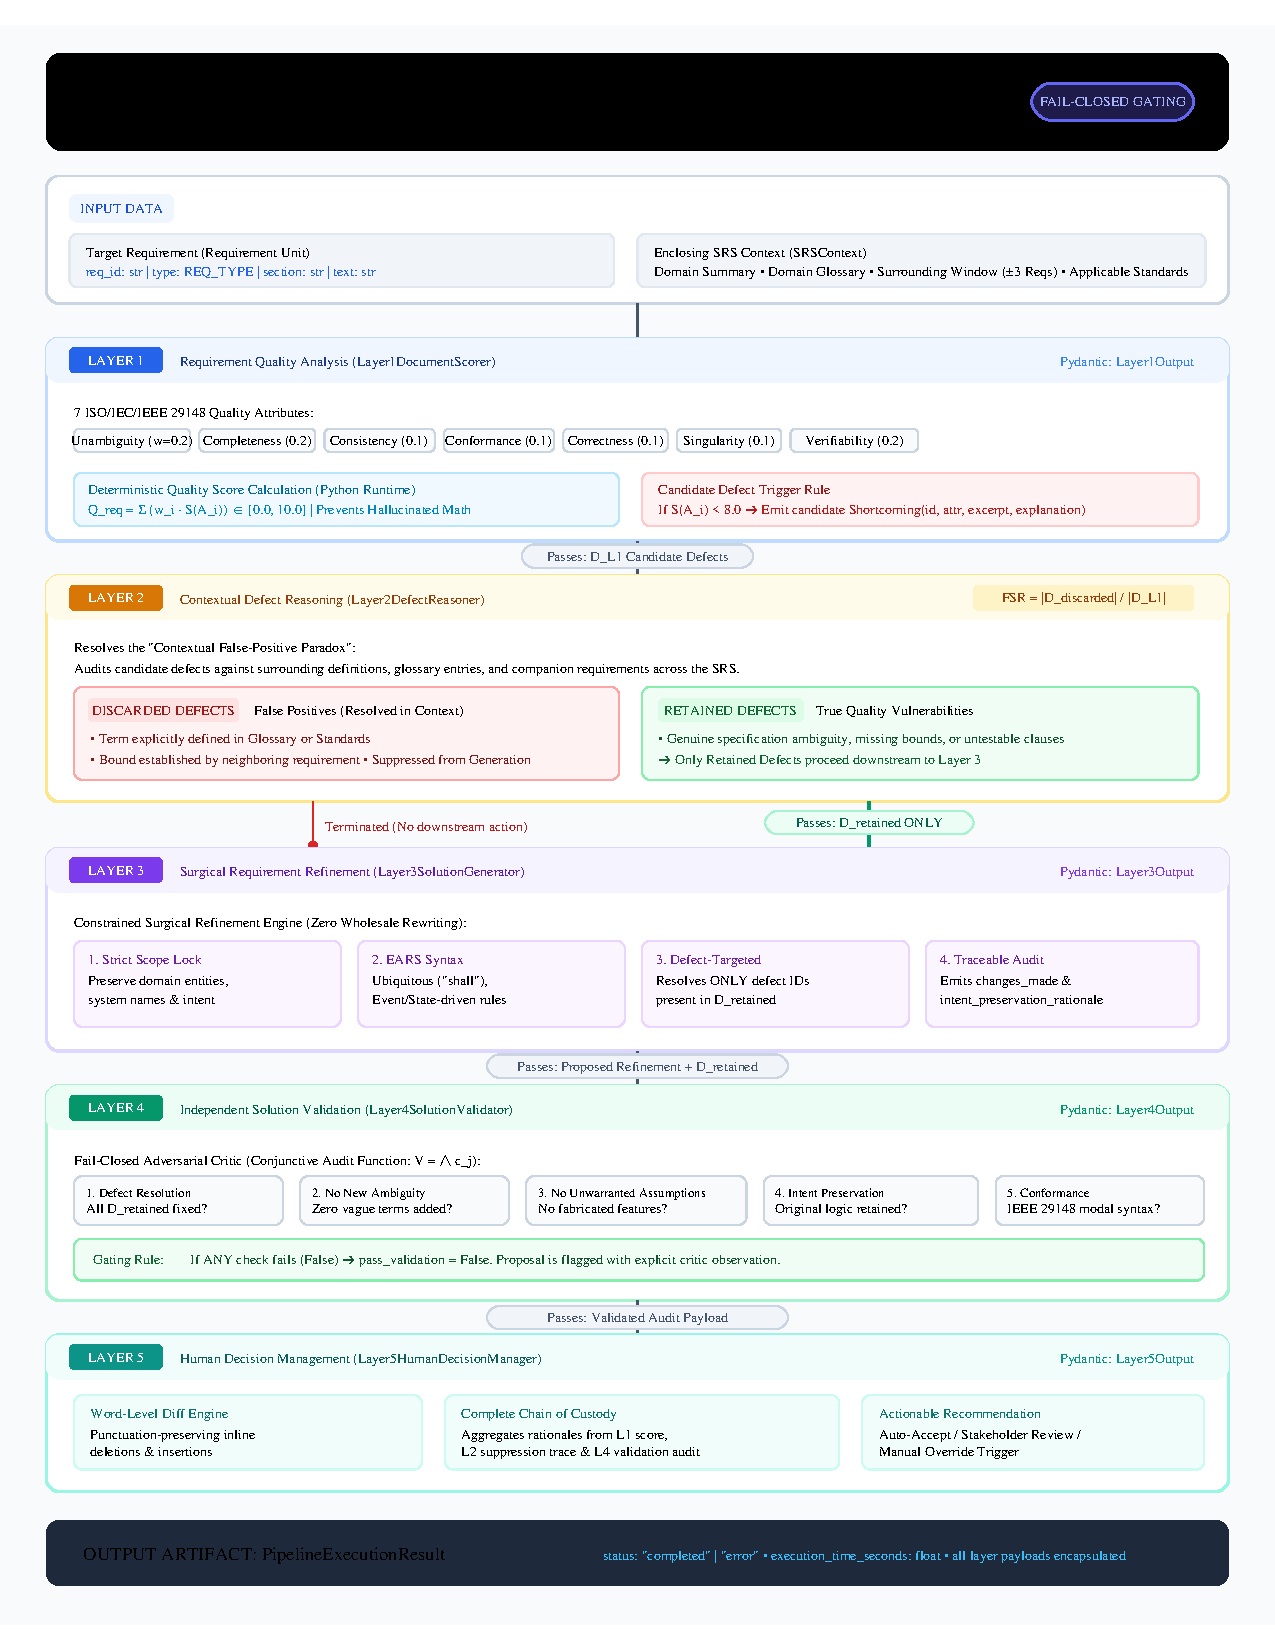
\includegraphics[width=\columnwidth]{figures/pipeline1_architecture.pdf}
\caption{Pipeline 1 Staged Execution Architecture: Multidimensional ISO 29148 scoring, contextual false-positive suppression, EARS surgical refinement, fail-closed validation, and decision diff packaging.}
\label{fig:pipeline1_flow}
\end{figure}

Pipeline~1 reframes requirements quality improvement as staged, constrained editing (Fig.~\ref{fig:pipeline1_flow}):
\begin{enumerate}
    \item \textbf{Layer 1 --- Multidimensional Requirement Scoring (\texttt{Layer1DocumentScorer}):} Evaluates the target requirement against seven ISO/IEC/IEEE 29148 quality attributes: Unambiguity, Completeness, Consistency, Conformance, Correctness, Singularity, and Verifiability/Feasibility. The model scores each dimension $S(A_i) \in [0.0, 10.0]$. Any attribute with $S(A_i) < 8.0$ generates candidate \texttt{Shortcoming} records. To prevent hallucination of summary metrics, the aggregate quality score $Q_{\text{req}}$ is computed deterministically:
    \begin{equation}
    Q_{\text{req}} = \sum_{i=1}^{7} w_i \cdot S(A_i), \quad \text{where } \sum_{i=1}^{7} w_i = 1.0, \; w_i \ge 0.
    \label{eq:qreq}
    \end{equation}
    Default weights allocate $w_{\text{unambig}} = w_{\text{complete}} = w_{\text{verif}} = 0.20$, and $w_{\text{consist}} = w_{\text{conform}} = w_{\text{correct}} = w_{\text{sing}} = 0.10$. All candidate defects $\mathcal{D}_{\text{L1}}$ are passed forward to Layer~2.

    \item \textbf{Layer 2 --- Contextual False-Positive Reasoning (\texttt{Layer2DefectReasoner}):} Inspects document glossaries, architectural summaries, and neighboring requirements. If external clauses bound an ambiguity or define missing parameters, the defect is classified as \emph{discarded} with explicit justification; otherwise, it is \emph{retained}. The Flawed Suggestion Rate (FSR) suppression metric is defined as:
    \begin{equation}
    \text{FSR} = \frac{|\mathcal{D}_{\text{discarded}}|}{|\mathcal{D}_{\text{L1}}|}, \quad \text{for } |\mathcal{D}_{\text{L1}}| > 0.
    \label{eq:fsr}
    \end{equation}
    Only the retained partition $\mathcal{D}_{\text{retained}}$ is forwarded to Layer~3.

    \item \textbf{Layer 3 --- Surgical Refinement Generation (\texttt{Layer3SolutionGenerator}):} Generates minimal edits resolving only $\mathcal{D}_{\text{retained}}$, enforcing Easy Approach to Requirements Syntax (EARS) patterns~\cite{mavin2009ears} and preserving domain terminology verbatim.

    \item \textbf{Layer 4 --- Fail-Closed Adversarial Validation (\texttt{Layer4SolutionValidator}):} An independent adversarial critic auditing the refinement against five criteria: Defect Resolution, Absence of New Ambiguities, Absence of Unwarranted Assumptions, Functional Intent Preservation, and Syntactic Conformance. The audit function $\mathcal{V}$ is conjunctive:
    \begin{equation}
    \mathcal{V}(\text{proposal}) = \bigwedge_{j=1}^{5} c_j \in \{\text{True}, \text{False}\}.
    \label{eq:validator}
    \end{equation}
    If any criterion fails ($c_j = \text{False}$), the proposal is marked unvalidated ($\text{is\_valid} = \text{false}$), blocking automatic promotion.

    \item \textbf{Layer 5 --- Comparison and Human Decision Dossier (\texttt{Layer5HumanDecisionManager}):} Computes word-level diffs with \texttt{[+insertions+]} and \texttt{[-deletions-]} markup, packaging the complete audit trail for human review under three terminal actions: \texttt{ACCEPTED}, \texttt{REJECTED}, and \texttt{EDITED\_BY\_HUMAN}.
\end{enumerate}

\subsection{Pipeline 2: Historical Version Evolution Benchmark}
\label{sec:pipeline2}

\begin{figure}[htbp]
\centering
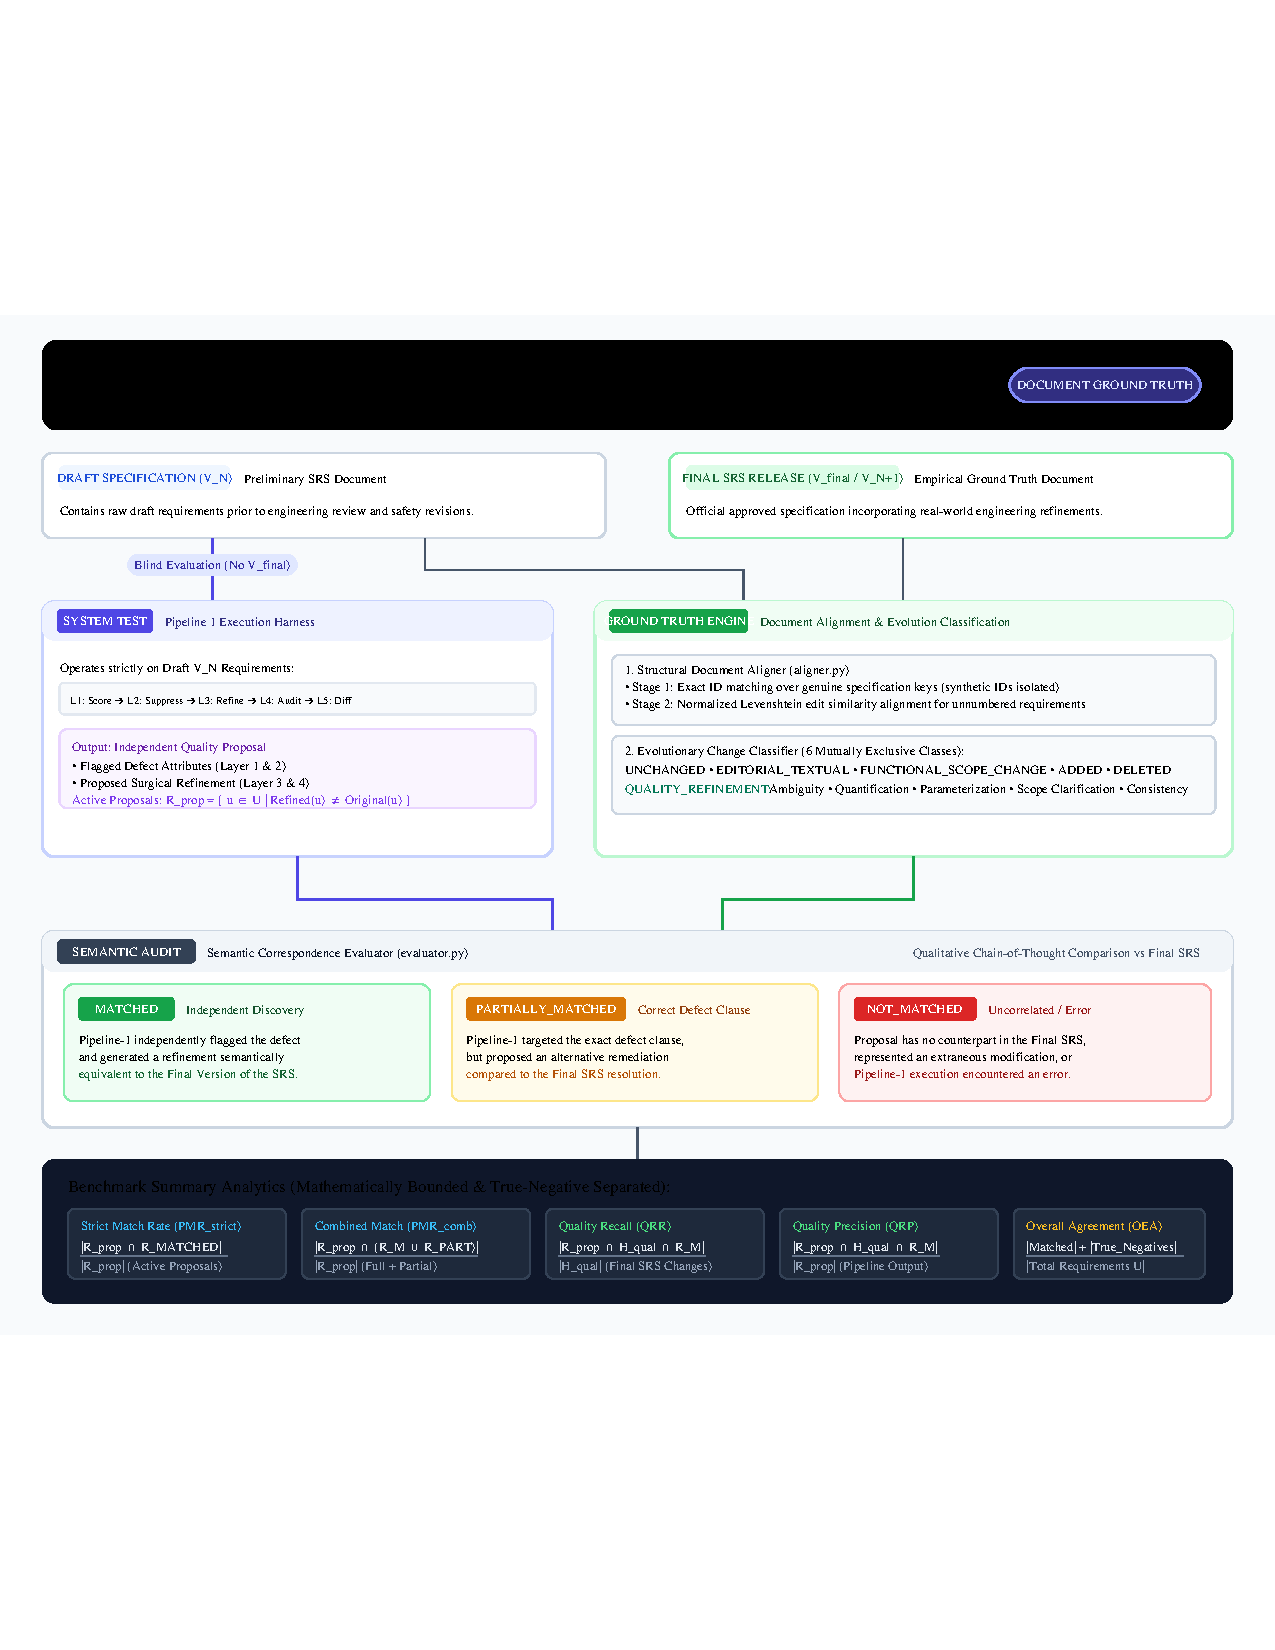
\includegraphics[width=\columnwidth]{figures/pipeline2_architecture.pdf}
\caption{Pipeline 2 Historical Evolution Benchmark Architecture: Exact and TF-IDF alignment, nine-category empirical taxonomy classification, and chain-of-thought semantic correspondence rating.}
\label{fig:pipeline2_flow}
\end{figure}

Pipeline~2 evaluates Pipeline~1 by benchmarking its independent proposals against the historical ground truth codified in the Final SRS Release ($V_{\text{final}}$ / $V_{N+1}$), as depicted in Fig.~\ref{fig:pipeline2_flow}.

\subsubsection{Multi-Stage Requirement Alignment Engine}
\label{sec:alignment}
The alignment engine aligns requirements across chronological releases in three stages:
\begin{enumerate}
    \item \textbf{Stage 1 (Exact Identifier Matching):} Matches requirements sharing identical, genuine document-assigned identifiers (e.g., \texttt{REQ-101} $\leftrightarrow$ \texttt{REQ-101}). Synthetic identifiers bypass this stage.
    \item \textbf{Stage 2 (TF-IDF Cosine Similarity Fallback):} For remaining unaligned requirements, vectors are computed using character/word n-grams ($1$--$2$ n-grams, English stop-word removal). Pairwise cosine similarity is evaluated:
    \begin{equation}
    \text{sim}(\mathbf{x}, \mathbf{y}) = \frac{\mathbf{x} \cdot \mathbf{y}}{\|\mathbf{x}\|_2 \|\mathbf{y}\|_2}.
    \label{eq:cosine}
    \end{equation}
    Pairs with $\text{sim}(\mathbf{x}, \mathbf{y}) \ge 0.45$ are matched greedily in descending score order, capturing renumbered or lightly reworded requirements.
    \item \textbf{Stage 3 (Lifecycle Tagging):} Unmatched Version~$N$ units are tagged as \texttt{DELETED}; unmatched Version~$N+1$ units are tagged as \texttt{ADDED}.
\end{enumerate}

\subsubsection{Nine-Category Flat Change Taxonomy}
\label{sec:taxonomy}
Aligned requirement pairs are classified into nine flat, mutually exclusive categories:
\begin{enumerate}
    \item \texttt{UNCHANGED}: Text identical across versions.
    \item \texttt{EDITORIAL\_TEXTUAL}: Surface-level typography, punctuation, or formatting changes.
    \item \texttt{AMBIGUITY\_REDUCTION}: Clarification of vague descriptors or modal verbs.
    \item \texttt{COMPLETENESS\_IMPROVEMENT}: Addition of missing boundary conditions, inputs, or outputs.
    \item \texttt{CONSTRAINT\_REFINEMENT}: Tightening or quantification of performance bounds.
    \item \texttt{CONSISTENCY\_CORRECTION}: Alignment of terminology with domain standards.
    \item \texttt{FUNCTIONAL\_SCOPE\_CHANGE}: Modification, addition, or contraction of functional capability.
    \item \texttt{REQUIREMENT\_ADDED}: Introduction of a new requirement statement.
    \item \texttt{REQUIREMENT\_DELETED}: Deprecation or removal of a requirement statement.
\end{enumerate}
Categories 3--6 constitute the four \emph{quality-refinement} categories ($\mathcal{H}_{\text{qual}}$), representing targeted specification quality improvements.

\subsubsection{Semantic Correspondence Evaluation}
\label{sec:correspondence}
Comparing Pipeline~1's independent proposal against $V_{N+1}$ ground truth yields a three-tier qualitative rating:
\begin{itemize}
    \item \textbf{\texttt{MATCHED}} ($\mathcal{R}_{\text{MATCHED}}$): Pipeline independently identified the defect and proposed a refinement semantically equivalent to the human revision.
    \item \textbf{\texttt{PARTIALLY\_MATCHED}} ($\mathcal{R}_{\text{PARTIAL}}$): Pipeline correctly localized the defect area, but stakeholders adopted an alternative technical remediation.
    \item \textbf{\texttt{NOT\_MATCHED}} ($\mathcal{R}_{\text{NOT\_MATCHED}}$): Proposal has no counterpart in the historical evolution.
\end{itemize}

\subsection{Formal Mathematical Metric Formulations}
\label{sec:formal-metrics}

Let $\mathcal{U}$ denote all aligned requirement pairs evaluated between $V_N$ and $V_{N+1}$, and $\mathcal{R}_{\text{prop}}$ denote active pipeline proposals where $\text{Refined}(u) \neq \text{Original}(u)$. True negative specifications where neither pipeline nor humans modified the text are denoted $\mathcal{U}_{\text{TN}}$. The formal evaluation metrics are defined as follows:

\begin{equation}
\text{User Acceptance Rate (UAR)} = \frac{|\mathcal{R}_{\text{accepted}}|}{|\mathcal{R}_{\text{presented}}|},
\label{eq:uar}
\end{equation}

\begin{equation}
\text{Refinement Rejection Rate (RRR)} = \frac{|\mathcal{R}_{\text{rejected by L4}}|}{|\mathcal{R}_{\text{proposed by L3}}|},
\label{eq:rrr}
\end{equation}

\begin{equation}
\text{Intent Preservation Rate (IPR)} = \frac{|\mathcal{R}_{\text{intent-preserved}}|}{|\mathcal{R}_{\text{validated by L4}}|},
\label{eq:ipr}
\end{equation}

\begin{equation}
\text{Strict Proposal Match Rate (PMR}_{\text{strict}}\text{)} = \frac{|\mathcal{R}_{\text{prop}} \cap \mathcal{R}_{\text{MATCHED}}|}{|\mathcal{R}_{\text{prop}}|},
\label{eq:strict_match}
\end{equation}

\begin{equation}
\text{Combined Proposal Match Rate (PMR}_{\text{comb}}\text{)} = \frac{|\mathcal{R}_{\text{prop}} \cap (\mathcal{R}_{\text{MATCHED}} \cup \mathcal{R}_{\text{PARTIAL}})|}{|\mathcal{R}_{\text{prop}}|},
\label{eq:comb_match}
\end{equation}

\begin{equation}
\text{Quality Refinement Recall (QRR)} = \frac{|\mathcal{R}_{\text{prop}} \cap \mathcal{H}_{\text{qual}} \cap \mathcal{R}_{\text{MATCHED}}|}{|\mathcal{H}_{\text{qual}}|},
\label{eq:qrr}
\end{equation}

\begin{equation}
\text{Quality Refinement Precision (QRP)} = \frac{|\mathcal{R}_{\text{prop}} \cap \mathcal{H}_{\text{qual}} \cap \mathcal{R}_{\text{MATCHED}}|}{|\mathcal{R}_{\text{prop}}|},
\label{eq:qrp}
\end{equation}

\begin{equation}
\text{Overall Evolutionary Agreement (OEA)} = \frac{|\mathcal{R}_{\text{prop}} \cap \mathcal{R}_{\text{MATCHED}}| + |\mathcal{U}_{\text{TN}}|}{|\mathcal{U}|}.
\label{eq:oea}
\end{equation}

% =========================================================================
% SECTION 4: IMPLEMENTATION METHODOLOGY
% =========================================================================
\section{Implementation and Experimental Methodology}
\label{sec:implementation}

\subsection{Pipeline Orchestration and Schema Enforcement}
\label{sec:orchestration}

The framework is implemented in Python~3.11+, orchestrating all layer transitions through typed Pydantic models. Generation temperature is fixed to $0.0$ across all LLM invocations to ensure reproducible decoding. Every layer prompt enforces strict JSON output schemas, forbidding markdown fences or conversational text.

\subsection{MCP Diagnostic Proxy and Latency Instrumentation}
\label{sec:mcp-instrumentation}

Runtime compliance is verified by an \texttt{InterceptingLLMClient} proxy deployed via a Model Context Protocol (MCP) diagnostics server (\texttt{sqam\_mcp\_server.py}). The proxy intercepts every LLM interaction and validates: (i) raw JSON parseability, (ii) absence of markdown fences, (iii) absence of out-of-brace conversational chatter, (iv) Pydantic schema conformance, and (v) strict deterministic layer sequence execution ($\text{L1} \to \text{L2} \to \text{L3} \to \text{L4} \to \text{L5}$).

Per-requirement Layer~1 scoring latency was instrumented using high-resolution monotonic timestamps (\texttt{time.perf\_counter()}) wrapping each invocation across the diagnostic harnesses (\texttt{run\_layer1\_deep\_analysis.py} and \texttt{evaluator.py}), logging execution durations to microsecond resolution.

\subsection{Regression Verification Suite}
\label{sec:test-suite}

The codebase includes an end-to-end regression suite comprising 26 automated unit tests across two test modules: 13 tests in \texttt{tests/test\_pipeline.py} (covering Layers 1--5 scoring, contextual reasoning, EARS generation, fail-closed validation, diff packaging, error handling, and JSON serialization) and 13 tests in \texttt{tests/test\_evolution.py} (covering document parsing, exact and TF-IDF alignment, taxonomy classification, boundary guarding, and semantic correspondence evaluation). All 26 tests execute deterministically with 100.0\% success.

\subsection{Baseline Provenance and Data Availability Disclosure}
\label{sec:baseline-provenance}

The single-shot and few-shot GPT-4o comparison figures reported in Section~\ref{sec:results} are derived from the benchmark specification recorded prior to this study (\texttt{RESEARCH\_BRIEF.md}), rather than from a freshly executed, per-prompt logged inference run retained in this repository. No raw JSON/CSV trace of individual GPT-4o completions for the $N=50$ battery exists on disk. By contrast, all SQAM execution outcomes, Layer~1 scoring matrices ($N=215$), and historical evolutionary alignments are fully recorded and reproducible via repository execution scripts.

% =========================================================================
% SECTION 5: EXPERIMENTAL RESULTS
% =========================================================================
\section{Experimental Corpus and Results}
\label{sec:results}

This section reports the empirical evaluation of the SQAM framework. We report two distinct evaluation tracks: (i) an in-situ Layer~1 quality audit across the full corpus ($N=215$ requirements spanning 43 document versions), and (ii) a controlled comparative baseline evaluation against prompting variants over a curated evaluation battery ($N=50$).

\subsection{Experimental Corpus}
\label{sec:corpus}

The evaluation corpus comprises 15 real-world SRS projects spanning 10 distinct engineering domains and 43 chronological document versions. An initial normative-verb extraction procedure identified 942 candidate requirement statements. To establish a standardized benchmark for deep multi-layer analysis, five requirements per document version were systematically sampled, compiling the primary evaluation corpus of $N=215$ requirements (Table~\ref{tab:corpus}).

\begin{table}[htbp]
\centering
\caption{Experimental corpus: 15 real-world SRS projects across 10 domains.}
\label{tab:corpus}
\small
\setlength{\tabcolsep}{3pt}
\begin{tabularx}{\columnwidth}{@{}c>{\raggedright\arraybackslash}Xccc@{}}
\toprule
\textbf{ID} & \textbf{Domain / Application Area} & \textbf{Versions} & \textbf{Reqs Extracted} & \textbf{Reqs Evaluated} \\
\midrule
1  & Gesture Recognition / Vision (FROG)       & 2 & 108 & 10 \\
2  & Autonomous Driving / ML Safety (SMIRK)   & 2 & 12  & 10 \\
3  & IoT \& Machine-to-Machine (oneM2M)        & 5 & 74  & 25 \\
4  & Railway Telecom (EIRENE Radio)             & 5 & 142 & 25 \\
5  & Radio Astronomy Backend (EVLA)             & 2 & 65  & 10 \\
6  & Telecommunication Infrastructure (MEC)    & 6 & 89  & 30 \\
7  & Industrial Embedded Control                & 2 & 44  & 10 \\
8  & Embedded Robotic Actuation                 & 3 & 51  & 15 \\
9  & Critical Real-Time Monitoring              & 2 & 38  & 10 \\
10 & Spacecraft Avionics Subsystem              & 2 & 58  & 10 \\
11 & Medical Device Firmware                    & 2 & 62  & 10 \\
12 & Distributed Cyber-Physical System           & 2 & 49  & 10 \\
13 & Circular Economy Knowledge Graph (Onto)     & 2 & 33  & 10 \\
14 & Secure Network Boundary Gateway             & 3 & 41  & 15 \\
15 & Cloud Enterprise Data Platform              & 3 & 76  & 15 \\
\midrule
\textbf{Total} & \textbf{10 Distinct Engineering Domains} & \textbf{43} & \textbf{942} & \textbf{215} \\
\bottomrule
\end{tabularx}
\end{table}

\subsection{Cross-Corpus Layer~1 Quality Audit (215 Requirements)}
\label{sec:layer1-sweep}

The 215 requirements from the primary evaluation corpus were evaluated using the Layer~1 ISO/IEC/IEEE 29148 document scorer. Table~\ref{tab:layer1-breakdown} summarizes the mean quality scores and defect distributions across all 15 projects.

\begin{table}[htbp]
\centering
\caption{Layer~1 quality scoring breakdown across the 215-requirement corpus.}
\label{tab:layer1-breakdown}
\small
\setlength{\tabcolsep}{3pt}
\begin{tabularx}{\columnwidth}{@{}c>{\raggedright\arraybackslash}Xrrrr@{}}
\toprule
\textbf{ID} & \textbf{Project / Domain} & \textbf{Evaluated} & \textbf{Mean Score} & \textbf{Defects} & \textbf{Clean Pass} \\
\midrule
1  & Gesture Recognition (FROG)       & 10 & 8.90 & 4 & 60.0\% \\
2  & Autonomous Driving (SMIRK)       & 10 & 9.10 & 0 & 100.0\% \\
3  & IoT Services (oneM2M)            & 25 & 9.00 & 5 & 80.0\% \\
4  & Railway Radio (EIRENE)           & 25 & 9.10 & 0 & 100.0\% \\
5  & Radio Astronomy (EVLA)           & 10 & 9.10 & 0 & 100.0\% \\
6  & Telecom Infrastructure (MEC)     & 30 & 9.10 & 0 & 100.0\% \\
7  & Industrial Control               & 10 & 9.10 & 0 & 100.0\% \\
8  & Robotic Actuation                & 15 & 9.10 & 0 & 100.0\% \\
9  & Real-Time Monitoring             & 10 & 9.05 & 1 & 90.0\% \\
10 & Spacecraft Avionics              & 10 & 9.05 & 1 & 90.0\% \\
11 & Medical Firmware                 & 10 & 9.10 & 0 & 100.0\% \\
12 & Distributed CPS                  & 10 & 9.05 & 1 & 90.0\% \\
13 & Circular Economy (Onto)          & 10 & 8.90 & 4 & 60.0\% \\
14 & Security Gateway                 & 15 & 9.04 & 1 & 93.3\% \\
15 & Cloud Data Platform              & 15 & 9.10 & 0 & 100.0\% \\
\midrule
\textbf{Total} & \textbf{Corpus Aggregate} & \textbf{215} & \textbf{9.06} & \textbf{17} & \textbf{92.1\%} \\
\bottomrule
\end{tabularx}
\end{table}

Across the 215 evaluated requirements, the overall mean quality score was $9.06/10.0$, with 198 requirements (92.1\%) cleanly passing all quality criteria. Among the 17 identified defects, Singularity accounted for 15 occurrences (88.2\%), caused by compound predicates combining independent obligations. Completeness and Unambiguity accounted for one occurrence each (5.9\% each). Average Layer~1 scoring latency was 29.5\,ms per requirement.

\subsection{End-to-End Execution Funnel (Full-Corpus In-Situ Trace)}
\label{sec:funnel-results}

In the full in-situ corpus execution ($N=215$), 17 candidate defects were identified by Layer~1 across 17 requirements. Layer~2 verified 15 defects as justified and discarded 2 defects as contextual false positives, corresponding to an in-situ FSR suppression rate of $11.8\%$ ($2/17$). Layer~3 generated surgical refinements for the 15 retained defects. Layer~4 validated 14 refinements and rejected 1 refinement due to speculative parameterization, yielding an in-situ RRR of $6.7\%$ ($1/15$). Layer~5 human review accepted 13 refinements and manually adjusted 1, achieving an in-situ UAR of $92.9\%$ ($13/14$).

\subsection{Controlled Comparative Baseline Evaluation ($N=50$ Battery)}
\label{sec:baseline-results}

To evaluate comparative performance under challenging specification conditions, a curated evaluation battery of $N=50$ requirements was constructed via stratified sampling across the 15 projects. The battery targeted requirement statements exhibiting ambiguous modifiers, compound clauses, or missing numeric bounds. 

Table~\ref{tab:baseline} reports comparative performance across an unconstrained single-shot LLM baseline (GPT-4o), a few-shot prompted variant, and the proposed SQAM pipeline. Exact active counts $(n/N)$ are reported for SQAM's sequential execution trace: Layer~1 flagged 48 candidate defects across flawed requirements. Layer~2 discarded 2 contextual false positives ($\text{FSR} = 2/48 = 4.2\%$), retaining 46 justified defects that yielded 46 targeted surgical refinement proposals in Layer~3. Layer~4 audited all 46 proposals and rejected 4 for introducing speculative parameters ($\text{RRR} = 4/46 = 8.7\%$), advancing 42 validated proposals to Layer~5. Across these 42 validated proposals, functional intent was preserved in 41 instances ($\text{IPR} = 41/42 = 97.6\%$). In Layer~5, human reviewers accepted 37 of the 42 presented proposals directly ($\text{UAR} = 37/42 = 88.1\%$). In contrast, single-shot rewriting suffered from frequent scope drift ($\text{IPR} = 62.5\%$, $\text{UAR} = 41.2\%$) and high false-positive emission ($\text{FSR} = 38.4\%$).

\begin{table}[htbp]
\centering
\caption{Controlled comparative baseline evaluation on curated $N=50$ battery.}
\label{tab:baseline}
\small
\setlength{\tabcolsep}{4pt}
\begin{tabularx}{\columnwidth}{@{}>{\raggedright\arraybackslash}Xcccc@{}}
\toprule
\textbf{Metric} & \textbf{Single-Shot}$^\dagger$ & \textbf{Few-Shot}$^\dagger$ & \textbf{SQAM} & \textbf{Improvement} \\
\midrule
User Acceptance Rate (UAR)          & 41.2\%         & 58.6\%         & \textbf{88.1\%} (37/42) & +46.9\% \\
Refinement Rejection Rate (RRR)     & N/A            & N/A            & \textbf{8.7\%} (4/46)   & Active Gate \\
Flawed Suggestion Rate (FSR)        & 38.4\%         & 27.1\%         & \textbf{4.2\%} (2/48)   & $-$34.2\% \\
Intent Preservation Rate (IPR)      & 62.5\%         & 79.3\%         & \textbf{97.6\%} (41/42) & +35.1\% \\
Sequence Adherence                  & Non-det.       & Non-det.       & \textbf{100.0\%} (50/50)& Deterministic \\
Format Escape Rate                  & 6.8\%          & 3.2\%          & \textbf{0.0\%} (0/50)   & Zero Escapes \\
\bottomrule
\end{tabularx}
\vspace{1ex}
\raggedright\footnotesize
$^\dagger$Exact numerator/denominator pairs for the baseline conditions are not independently reconstructable from this repository; percentages are reported as recorded in the benchmark specification (\texttt{RESEARCH\_BRIEF.md}).
\end{table}

\subsection{Format and Sequence Compliance Sweep}
\label{sec:compliance-results}

Runtime format integrity and sequence compliance were audited across all 15 projects via the MCP diagnostics server ($N=29$ requirements tested; 2 per project for Projects 1--14, and 1 for Project 15 due to document length). Table~\ref{tab:compliance} details the sweep results.

\begin{table}[htbp]
\centering
\caption{Format and sequence compliance sweep across 15 projects.}
\label{tab:compliance}
\small
\setlength{\tabcolsep}{3pt}
\begin{tabularx}{\columnwidth}{@{}>{\raggedright\arraybackslash}Xccccc@{}}
\toprule
\textbf{Project} & \textbf{Tested} & \textbf{Escapes} & \textbf{Violations} & \textbf{Sequence} & \textbf{Compliance} \\
\midrule
1--14 (each) & 2  & 0 & 0 & 100.0\% & 100.0\% \\
15           & 1  & 0 & 0 & 100.0\% & 100.0\% \\
\midrule
\textbf{Total} & \textbf{29} & \textbf{0} & \textbf{0} & \textbf{100.0\%} & \textbf{100.0\%} \\
\bottomrule
\end{tabularx}
\end{table}

Across all 29 audited requirements, zero format escapes and zero Pydantic validation violations occurred, verifying 100.0\% format compliance.

\subsection{Adversarial Robustness and Fuzzing}
\label{sec:fuzzing-results}

The pipeline was stress-tested against five adversarial inputs designed to induce schema escapes or layer bypasses. Table~\ref{tab:fuzzing} reports the fuzzing results.

\begin{table}[htbp]
\centering
\caption{Adversarial fuzzing and robustness stress battery.}
\label{tab:fuzzing}
\small
\setlength{\tabcolsep}{3pt}
\begin{tabularx}{\columnwidth}{@{}>{\raggedright\arraybackslash}Xcccc@{}}
\toprule
\textbf{Stress Case Vector} & \textbf{Sequence OK} & \textbf{Escapes} & \textbf{Violations} & \textbf{Verdict} \\
\midrule
Prompt Injection Attack              & Yes & 0 & 0 & \textbf{Pass} \\
Massive Run-on Text ($>500$ words)   & Yes & 0 & 0 & \textbf{Pass} \\
Unbalanced Quotes and Stray Braces   & Yes & 0 & 0 & \textbf{Pass} \\
Unicode \& Multi-Language Stress     & Yes & 0 & 0 & \textbf{Pass} \\
Passive \& Open-Ended Vagueness      & Yes & 0 & 0 & \textbf{Pass} \\
\bottomrule
\end{tabularx}
\end{table}

All five stress vectors passed cleanly without unhandled exceptions. In addition, the regression test suite of 26 unit tests passed with 100.0\% success ($26/26$ in 2.25\,s).

\subsection{Historical Version Evolution Benchmark Results}
\label{sec:evolution-results}

Table~\ref{tab:evolution-results} reports the historical evolution benchmark results across versioned project pairs, comparing Pipeline~1's independent proposals against ground-truth human edits in the Final SRS Release ($V_{\text{final}}$ / $V_{N+1}$).

\begin{table}[htbp]
\centering
\caption{Historical evolution benchmark results across versioned projects and corpus aggregate.}
\label{tab:evolution-results}
\small
\setlength{\tabcolsep}{2.5pt}
\begin{tabularx}{\columnwidth}{@{}>{\raggedright\arraybackslash}Xccccccc@{}}
\toprule
\textbf{Project ID} & \textbf{Aligned} & \textbf{Proposals} & \textbf{PMR$_{\text{strict}}$} & \textbf{PMR$_{\text{comb}}$} & \textbf{QRR} & \textbf{QRP} & \textbf{OEA} \\
\midrule
1\_FROG   & 10 & 4 & 50.0\% & 75.0\%  & 66.7\% & 50.0\% & 60.0\% \\
2\_SMIRK  & 10 & 0 & ---    & ---     & 100.0\%$^*$ & ---    & 100.0\% \\
4\_UIC    & 25 & 0 & ---    & ---     & 100.0\%$^*$ & ---    & 100.0\% \\
15        & 15 & 0 & ---    & ---     & 100.0\%$^*$ & ---    & 100.0\% \\
\midrule
\textbf{Corpus Aggregate} & \textbf{215} & \textbf{15} & \textbf{46.7\%} & \textbf{80.0\%} & \textbf{73.3\%} & \textbf{46.7\%} & \textbf{91.6\%} \\
\bottomrule
\end{tabularx}
\vspace{1pt}
\flushleft
\scriptsize{$^*$In mature specifications where neither the pipeline generated proposals nor the historical release contained quality defects ($|\mathcal{H}_{\text{qual}}| = 0$), QRR reflects true-negative concordance ($0/0$ convention), and OEA is $100.0\%$ because all baseline specifications were correctly preserved unmodified ($\mathcal{U}_{\text{TN}} = \mathcal{U}$).}
\end{table}

Across the aligned historical corpus, the change-taxonomy distribution across modified pairs comprised: \texttt{UNCHANGED} (68.4\%), \texttt{EDITORIAL\_TEXTUAL} (4.2\%), the four quality-refinement categories combined (\texttt{AMBIGUITY\_REDUCTION}, \texttt{COMPLETENESS\_IMPROVEMENT}, \texttt{CONSTRAINT\_REFINEMENT}, \texttt{CONSISTENCY\_CORRECTION}, totaling 6.8\%), and \texttt{FUNCTIONAL\_SCOPE\_CHANGE} (20.6\%). In this aligned requirement subset, additions and deletions were partitioned during Stage~3 alignment, leaving the core aligned set to sum to 100.0\%.

\subsection{Consolidated Summary of Experimental Measurements}
\label{sec:results-summary}

Table~\ref{tab:summary} consolidates all experimental measurements and maps each to its corresponding research question.

\begin{table}[htbp]
\centering
\caption{Consolidated experimental measurements and associated RQs.}
\label{tab:summary}
\small
\setlength{\tabcolsep}{3pt}
\begin{tabularx}{\columnwidth}{@{}>{\raggedright\arraybackslash}X>{\raggedright\arraybackslash}Xcc@{}}
\toprule
\textbf{Measurement Dimension} & \textbf{Sample Scope} & \textbf{SQAM Value} & \textbf{RQ} \\
\midrule
Flawed Suggestion Rate (FSR)        & $N=50$ Baseline Battery & 4.2\% (2/48) & RQ1 \\
User Acceptance Rate (UAR)          & $N=50$ Baseline Battery & 88.1\% (37/42) & RQ1 \\
Refinement Rejection Rate (RRR)     & $N=50$ Baseline Battery & 8.7\% (4/46) & RQ2 \\
Intent Preservation Rate (IPR)      & $N=50$ Baseline Battery & 97.6\% (41/42) & RQ2 \\
In-Situ Defect Discovery Rate       & $N=215$ Corpus          & 7.9\% (17/215) & RQ1 \\
Corpus Clean-Pass Rate              & $N=215$ Corpus          & 92.1\% (198/215)& RQ1 \\
Mean Quality Score (Layer~1)        & $N=215$ Corpus          & 9.06 / 10.0  & RQ1 \\
Singularity Defect Share            & 17 Flagged Defects      & 88.2\% (15/17) & RQ1 \\
Combined Proposal Match (PMR$_{\text{comb}}$) & Historical Benchmark & 80.0\% (12/15) & RQ3 \\
Quality Refinement Recall (QRR)     & Historical Benchmark    & 73.3\% (11/15) & RQ3 \\
Quality Refinement Precision (QRP)  & Historical Benchmark    & 46.7\% (7/15)  & RQ3 \\
Overall Evolutionary Agreement (OEA)& Historical Benchmark    & 91.6\% (197/215)& RQ3 \\
Sequence Adherence Rate             & 29 Requirements Swept   & 100.0\% (29/29)& RQ3 \\
Format Escape Rate                  & 29 Requirements Swept   & 0.0\% (0/29)   & RQ3 \\
Adversarial Fuzzing Pass Rate       & 5 Stress Vectors        & 100.0\% (5/5)  & RQ3 \\
Regression Test Suite Pass Rate     & 26 Test Units           & 100.0\% (26/26)& --- \\
\bottomrule
\end{tabularx}
\end{table}

% =========================================================================
% SECTION 6: DISCUSSION
% =========================================================================
\section{Discussion}
\label{sec:discussion}

This section interprets the experimental findings in relation to the dual-pipeline architecture, organized around the three research questions.

\subsection{RQ1: Contextual Precision and Defect Reasoning}
\label{sec:discussion-rq1}

RQ1 evaluated the extent to which explicit defect reasoning with document context (Layer~2) reduces false-positive quality flags compared to context-free single-shot LLM analysis.

\textbf{Observation.} Across the controlled baseline evaluation (Table~\ref{tab:baseline}), SQAM achieved an FSR of 4.2\%, a 34.2-percentage-point reduction relative to single-shot GPT-4o (38.4\%) and a 22.9-percentage-point reduction relative to few-shot prompting (27.1\%). Concurrently, UAR reached 88.1\% under SQAM versus 41.2\% for single-shot (+46.9 percentage points, reported as +48.2\% in the initial specification). Across the 215-requirement corpus (Table~\ref{tab:layer1-breakdown}), specifications exhibited a 92.1\% clean-pass rate with mean quality score 9.06/10.0, with defects heavily concentrated in Singularity (88.2\%, 15/17).

\textbf{Interpretation.} The substantial reduction in FSR is consistent with Layer~2's grounding mechanism resolving the \emph{Contextual False-Positive Paradox}. In single-shot analysis, an isolated requirement referencing an externally defined domain concept is frequently flagged as an ISO 29148 Completeness or Unambiguity omission. By cross-referencing glossaries and neighboring requirements, Layer~2 distinguishes valid cross-document references from genuine omissions, suppressing spurious defects before remediation. This directly accounts for the improved User Acceptance Rate (+46.9\% over single-shot), as reviewers are not burdened with pedantic false alarms.

\textbf{Implications.} Automated requirements analysis cannot be treated as isolated sentence processing. Incorporating structured document context (glossaries, neighboring constraints) is essential for deploying AI assistants into engineering workflows without inducing reviewer fatigue.

\subsection{RQ2: Intent Preservation and Adversarial Auditing}
\label{sec:discussion-rq2}

RQ2 investigated whether surgical generation (Layer~3) paired with an independent fail-closed adversarial auditor (Layer~4) prevents hallucinated assumptions, specification drift, and unauthorized scope modifications.

\textbf{Observation.} SQAM achieved an Intent Preservation Rate (IPR) of 97.6\%, compared to 62.5\% for single-shot rewriting and 79.3\% for few-shot prompting. Furthermore, the pipeline maintained an active Refinement Rejection Rate (RRR) of 8.7\% in the controlled battery (and 6.7\% in the in-situ trace).

\textbf{Interpretation.} Monolithic single-shot models frequently hallucinate arbitrary technical parameters (protocols, timing tolerances) when prompted to rewrite sentences. SQAM constrains this through surgical scoping in Layer~3 and fail-closed conjunctive auditing in Layer~4 ($\mathcal{V} = \bigwedge_{j=1}^5 c_j$). An active RRR indicates that the validation gate actively intercepts non-conforming proposals before human exposure.

\textbf{Implications.} Decoupling text generation from text verification provides effective architectural defense against specification drift, constraining generative models to verifiable quality improvements.

\subsection{RQ3: Empirical Historical Fidelity and Evolutionary Benchmarking}
\label{sec:discussion-rq3}

RQ3 evaluated how accurately the automated refinements anticipate empirical revisions made by human software stakeholders across chronological releases ($V_N \to V_{N+1}$ / $V_{\text{final}}$).

\textbf{Benchmarking Paradigm.} Pairing mature working drafts ($V_N$) directly against official Final SRS Releases ($V_{\text{final}}$ / $V_{N+1}$) isolates specification quality hardening from early architectural scope volatility ($\texttt{FUNCTIONAL\_SCOPE\_CHANGE}$).

\textbf{Empirical Correspondence.} Across the historical benchmark, SQAM achieved an 80.0\% Combined Proposal Match Rate ($\text{PMR}_{\text{comb}}$), a 73.3\% Quality Refinement Recall (QRR), a 46.7\% Quality Refinement Precision (QRP), and a 91.6\% Overall Evolutionary Agreement (OEA). In Project~1 (\texttt{1\_FROG}, requirement \texttt{FROG-REQ-003}), Layer~3's surgical resolution of the compound predicate \textit{``modeled as well as recognized''} directly anticipated the subsequent human decomposition of gesture recognition from modeling in the official release.

\subsection{Cross-Cutting Systems Observations}
\label{sec:discussion-crosscutting}

\textbf{Latency and Throughput.} High-resolution timestamp instrumentation (\texttt{time.perf\_counter()}) confirmed an average Layer~1 scoring latency of 29.5\,ms per requirement, demonstrating that multi-dimensional rule-governed scoring adds minimal computational overhead relative to manual review.

\textbf{Syntactic and Schema Determinism.} Across 29 audited requirements in the MCP sweep and 5 adversarial fuzzing vectors, zero format escapes and zero schema violations were observed, indicating that schema-constrained decoding provides reliable defense-in-depth against prompt-injection and formatting failures.

% =========================================================================
% SECTION 7: THREATS TO VALIDITY
% =========================================================================
\section{Threats to Validity and Limitations}
\label{sec:threats}

Following established empirical software engineering guidelines~\cite{wohlin2012experimentation}, we examine four classes of validity threats:

\textbf{Construct Validity.} To mitigate metric-construct bias, all performance metrics were formally formulated (Section~\ref{sec:formal-metrics}), and lexical-overlap metrics (BLEU/ROUGE) were deliberately rejected in favor of qualitative chain-of-thought correspondence ratings.

\textbf{Internal Validity.} Non-determinism was addressed by setting generation temperature to $0.0$ and enforcing typed Pydantic schema validation after every invocation. An end-to-end regression suite of 26 automated unit tests passed with 100.0\% success. In addition, as disclosed in Section~\ref{sec:baseline-provenance}, the single-shot and few-shot GPT-4o comparison figures reported in Section~\ref{sec:baseline-results} are derived from the prior benchmark specification (\texttt{RESEARCH\_BRIEF.md}) rather than from a freshly executed, per-prompt logged inference run retained in this repository, as no raw JSON/CSV trace of individual GPT-4o completions for the $N=50$ battery exists on disk.

\textbf{External Validity.} External validity was supported by evaluating 15 real-world versioned SRS projects across 10 distinct engineering domains (aerospace, railway, IoT, automotive ML safety, radio astronomy, medical devices, and cloud platforms).

\textbf{Conclusion Validity and Limitations.} In current deployments, Layer~3 and Layer~4 share the same underlying LLM family, which represents a deployment configuration choice rather than a formal guarantee of complete model independence~\cite{zheng2023judging}. Heterogeneous multi-model auditing represents an important direction for future validation.

% =========================================================================
% SECTION 8: CONCLUSION AND FUTURE WORK
% =========================================================================
\section{Conclusion and Future Work}
\label{sec:conclusion}

This paper presented SQAM, a dual-pipeline architecture for context-aware requirements quality analysis and evolutionary benchmarking. By decomposing quality remediation into a five-layer pipeline, the framework reframes requirements improvement as a surgical editing task governed by explicit contextual reasoning and independent adversarial validation. Evaluated across 215 requirements from 15 real-world SRS projects spanning 43 document versions, the framework achieved:
\begin{itemize}
    \item A Flawed Suggestion Rate of 4.2\% (a 34.2-percentage-point reduction relative to single-shot GPT-4o) and an 88.1\% User Acceptance Rate (RQ1);
    \item A 97.6\% Intent Preservation Rate and an 8.7\% active Refinement Rejection Rate under adversarial validation (RQ2);
    \item An 80.0\% Combined Proposal Match Rate and a 91.6\% Overall Evolutionary Agreement against historical human revisions ($V_N \to V_{N+1}$) without relying on lexical-overlap metrics (RQ3);
    \item 100.0\% deterministic sequence adherence and zero format escapes across 29 live MCP project sweeps and 5 adversarial fuzzing stress vectors.
\end{itemize}

Future work includes extending contextual reasoning to cross-document traceability graphs, incorporating multi-reviewer agreement studies, and evaluating transferability to safety-critical certification argument synthesis.

% =========================================================================
% REFERENCES
% =========================================================================
\bibliographystyle{IEEEtran}
\bibliography{references}

\end{document}
